\documentclass{article}

\usepackage{tikz} 
\usetikzlibrary{matrix}


\begin{document}


\begin{tikzpicture}
    \draw (0,0) --(1,2);
\end{tikzpicture}

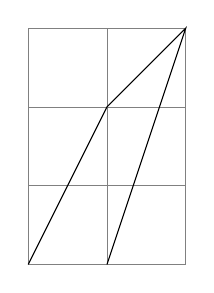
\begin{tikzpicture}
    \draw[help lines] (0,0) grid (2,3);
    \draw (0,0) --(1,2) -- (2,3) -- (1,0);
\end{tikzpicture}

\begin{tikzpicture}[xscale=2.5,yscale=0.5]
    \draw (0,0) -- (1,1);
\end{tikzpicture}

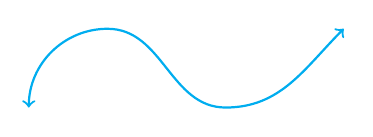
\begin{tikzpicture}
    \draw [<->,thick, cyan] (0,0) to [out=90,in=180] (1,1)
    to [out=0,in=180] (2.5,0) to [out=0,in=-135] (4,1) ;
\end{tikzpicture}

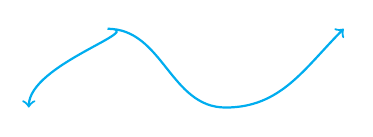
\begin{tikzpicture}
    \draw [<->,thick, cyan] (0,0) to [out=90,in=0] (1,1)
    to [out=0,in=180] (2.5,0) to [out=0,in=-135] (4,1) ;
\end{tikzpicture}

\begin{tikzpicture}
    \node[inner sep=0pt] (toad_rgb) at (0,0)
    {\includegraphics[width=.25\textwidth]{images/toad_rgb.png}};
    \node[inner sep=0pt] (toad_r) at (3,0)
    {\includegraphics[width=.25\textwidth]{images/toad_r.png}};
    \node[inner sep=0pt] (toad_g) at (6,0)
    {\includegraphics[width=.25\textwidth]{images/toad_g.png}};
    \node[inner sep=0pt] (toad_b) at (9,0)
    {\includegraphics[width=.25\textwidth]{images/toad_b.png}};
\end{tikzpicture}

\begin{tikzpicture}
    \node[inner sep=0pt] (toad_rgb) at (0,0)
    {\includegraphics[width=.18\textwidth]{images/toad_rgb.png}};
    \node[inner sep=0pt] (toad_r) at (2.5,0)
    {\includegraphics[width=.18\textwidth]{images/toad_r.png}};
    \node[inner sep=0pt] (toad_g) at (5,0)
    {\includegraphics[width=.18\textwidth]{images/toad_g.png}};
    \node[inner sep=0pt] (toad_b) at (7.5,0)
    {\includegraphics[width=.18\textwidth]{images/toad_b.png}};
    
    \draw [->] (toad_rgb.south) to [out=355, in=185] (toad_r.south);
    \draw [->] (toad_rgb.south) to [out=350, in=190] (toad_g.south);
    \draw [->] (toad_rgb.south) to [out=345, in=195] (toad_b.south);

    \draw [red] (7.5, 0.05) -- (7.6, 0.05) -- (7.6,-0.05) -- (7.5, -0.05) -- (7.5, 0.05);

    %\node (10.0,0.0) {$$\begin{bmatrix} 1 & 1 \\ 2 & 2 \end{bmatrix}$$};
    \matrix [matrix of nodes,row sep=-1ex, column sep=-1ex] (toad_mat) at (10.0, 0.0)
    {
        5 & 7 & 10 & 10 & 11 & 4 \\
        6 & 8 & 8 & 10 & 10 & 5 \\
        5 & 6 & 8 & 8 & 7 & 4 \\
        6 & 5 & 6 & 5 & 7 & 5 \\
        6 & 6 & 4 & 5 & 4 & 4 \\
        5 & 5 & 4 & 2 & 3 & 6  \\  };

    \draw [->] (7.6, 0.05) -- (toad_mat.north west);
    \draw [->] (7.6,-0.05) -- (toad_mat.south west);

    % draw matrix frame, how stupid I need to write it manually.
    \draw ([shift={(0.15, 0.0)}]toad_mat.north west) -- 
        ([shift={(0.05, 0.0)}]toad_mat.north west) --
        ([shift={(0.05, 0.0)}]toad_mat.south west) --
        ([shift={(0.15, 0.0)}]toad_mat.south west);

    \draw ([shift={(-0.15, 0.0)}]toad_mat.north east) -- 
        ([shift={(-0.05, 0.0)}]toad_mat.north east) --
        ([shift={(-0.05, 0.0)}]toad_mat.south east) --
        ([shift={(-0.15, 0.0)}]toad_mat.south east);

    \node at ([shift={(0.0, 0.2)}]toad_rgb.north) {RGB};
    \node at ([shift={(0.0, 0.2)}]toad_r.north) {R};
    \node at ([shift={(0.0, 0.2)}]toad_g.north) {G};
    \node at ([shift={(0.0, 0.2)}]toad_b.north) {B};
    \node at ([shift={(0.0, 0.2)}]toad_mat.north) {matrix of the crop};
    

    %\draw[help lines] (0,0) grid (10,-10);
\end{tikzpicture}

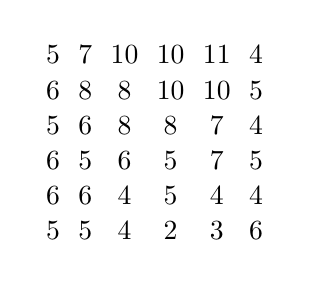
\begin{tikzpicture}
    %\matrix [matrix of nodes,row sep=-\pgflinewidth,column 6/.style={nodes={rectangle,draw,minimum width=3em}}]
    \matrix [matrix of nodes,row sep=-\pgflinewidth]
    {
        5 & 7 & 10 & 10 & 11 & 4 \\
        6 & 8 & 8 & 10 & 10 & 5 \\
        5 & 6 & 8 & 8 & 7 & 4 \\
        6 & 5 & 6 & 5 & 7 & 5 \\
        6 & 6 & 4 & 5 & 4 & 4 \\
        5 & 5 & 4 & 2 & 3 & 6  \\  };
\end{tikzpicture}
    

\end{document}
